
	\chapter{Projektplan}
	
	\section{Projektarbejdet}
	Der vil blive arbejdet på projektet alle hver dage fra 8.15-16.00. Der kommer dog dage med undervisning sideløbende med projektarbejdet, så nogle dage ville denne arbejdstid formindskes. \\
	
	\section{Projektplan}
	Her er et første udkast til projektplanen.
	\begin{figure}[h!]
		\centering
		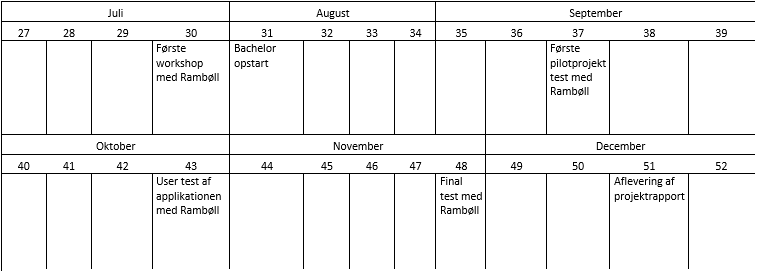
\includegraphics[width=0.9\linewidth]{Projektplan/Projektplan}
	\end{figure}

	\section{Projektstyring}

	Projektet vil blive styret igennem Scrum. Her vil blive arbejdet i sprints af 14 dage. Der vil blive brugt en online scrum værktøj til dette som f.eks. Zenhub plugin'et til github. Github vil også blive brugt til versions styring af kode og dokumenter. \\
	Der vil der udover være et møde med vejleder hver 14. dag. \\

	
	\section{Eksperimenter \& Teknologier}
	Der vil blive indsamlet viden til opbygningen af applikationen gennem workshops med den afdeling hos Rambøll vi skal udvikle for.\\
	Vi vil komme til at se hvordan de registrer i dag, hvilke informationer de bruger og hvilke andre behov de har.\\
	Disse workshops vil også blive holdt løbende med udviklingen af applikationen, for at teste og forbedre applikationen, så den er skræddersyet til deres behov. \newline
	Applikationen vil blive udviklet i Xarmarin, som er et cross platform plugin til Visual Studio, der gør det muligt at deployere koden til både iOS og Android.\\
	Dette valg er taget, da der ikke har været muligheder for at fremskaffe to Macbooks til udvikling. Da det er Rambølls ønske at få en applikation udviklet til iOS platformen er Xarmarin den bedste løsning indenfor de ressourcer vi har til rådighed. 

